\documentclass[11pt,a4paper]{article}

\usepackage[T1]{fontenc}
\usepackage[utf8]{inputenc}
\usepackage{mathptmx}
\usepackage[margin=2.5cm,top=2.6cm,bottom=2.6cm]{geometry}
\usepackage{graphicx}
\usepackage{booktabs}
\usepackage{longtable}
\usepackage{array}
\usepackage{xcolor}
\usepackage{titlesec}
\usepackage{enumitem}
\usepackage{amsmath}
\usepackage{amssymb}
\usepackage{fancyhdr}
\usepackage{caption}
\usepackage{tcolorbox}
\usepackage{microtype}
\usepackage[hidelinks]{hyperref}

\definecolor{inkblue}{HTML}{2C5F7C}
\definecolor{inkred}{HTML}{A85751}
\definecolor{inkgreen}{HTML}{3E7A5E}
\definecolor{inkwarn}{HTML}{B07A2E}
\definecolor{soft}{HTML}{6B6B6B}
\definecolor{panelbg}{HTML}{F6F7F8}

\titleformat{\section}{\Large\bfseries\color{inkblue}}{\thesection}{0.7em}{}
\titleformat{\subsection}{\large\bfseries}{\thesubsection}{0.7em}{}
\titleformat{\subsubsection}{\normalsize\bfseries\itshape}{\thesubsubsection}{0.7em}{}
\titlespacing*{\section}{0pt}{2.4ex plus 1ex minus .2ex}{1.4ex plus .2ex}

\captionsetup{font=small,labelfont={bf,color=inkblue},width=0.94\textwidth}
\setlist{itemsep=2pt,parsep=0pt,topsep=4pt}

\pagestyle{fancy}
\fancyhf{}
\fancyhead[L]{\footnotesize\color{soft}Dual Neprilysin / DPP-IV Inhibitor Discovery}
\fancyhead[R]{\footnotesize\color{soft}\thepage}
\renewcommand{\headrulewidth}{0.3pt}
\renewcommand{\headrule}{\hbox to\headwidth{\color{soft}\leaders\hrule height \headrulewidth\hfill}}

\newtcolorbox{keybox}[1][]{
  colback=panelbg, colframe=inkblue, boxrule=0.9pt, arc=2pt,
  left=8pt, right=8pt, top=6pt, bottom=6pt, #1}

\newtcolorbox{warnbox}[1][]{
  colback=white, colframe=inkwarn, boxrule=0.9pt, arc=2pt,
  left=8pt, right=8pt, top=6pt, bottom=6pt, #1}

\newcommand{\ang}{\text{\AA}}

\begin{document}

% ======================================================================
\begin{titlepage}
\centering
\vspace*{2.2cm}

{\color{soft}\large TECHNICAL REPORT}

\vspace{1.2cm}

{\Huge\bfseries\color{inkblue} Computational Discovery of a\\[0.3cm] Dual Neprilysin / DPP-IV Inhibitor}

\vspace{0.9cm}

{\Large A structure-based virtual screening pipeline for type 2 diabetes\\[0.2cm]
in patients at risk of heart failure with reduced ejection fraction}

\vspace{2.2cm}

{\large\bfseries Mohammed Mujtaba Shahnawaz Khan}

\vspace{0.4cm}

{\color{soft} B.Pharm, University of Mumbai \\
MSc Chemical Sciences and Instrumentation, Nanyang Technological University}

\vspace{2.4cm}

\begin{minipage}{0.86\textwidth}
\small
\begin{warnbox}
\textbf{Scope and provenance.} This report documents a virtual screening
methodology developed during the author's final-year undergraduate research
project. The original scripts and intermediate datasets were not preserved
under version control, and this document is therefore a reconstruction of the
methodology rather than a record of a specific set of results. Numerical values
presented in figures and tables are illustrative of how the pipeline behaves,
and are labelled as such throughout. No compound described here has been
synthesised or biologically assayed.

\smallskip
In the original project, machine learning model training and generative
expansion of the scaffold libraries were carried out by a doctoral colleague
rather than by the author. Section~\ref{sec:ml} explains that component in full
for the benefit of readers wishing to reproduce the work, and flags this
attribution where relevant.
\end{warnbox}
\end{minipage}

\vfill

{\small\color{soft}
Accompanying code and documentation:\\
\texttt{github.com/SupremeMaxitout/nep-dpp4-dual-inhibitor-screen}\\[0.3cm]
Version 1.0 \quad\textbullet\quad September 2026}

\end{titlepage}

% ======================================================================
\tableofcontents
\newpage

% ======================================================================
\section*{Summary}
\addcontentsline{toc}{section}{Summary}

Patients with type 2 diabetes and heart failure with reduced ejection fraction
(HFrEF) currently require separate drugs for each condition. A single molecule
inhibiting both neprilysin, a validated heart failure target, and dipeptidyl
peptidase-IV, a validated glycaemic target, would reduce pill burden and remove
a drug-drug interaction surface.

This report describes a computational pipeline designed to identify such
molecules. It proceeds in six stages: preparation and validation of the target
structures, construction of bioactivity-filtered compound libraries, primary
docking with rescoring, cross-docking to identify compounds active at both
targets, extraction and constrained enumeration of shared molecular scaffolds,
and counter-screening against the antitargets whose inhibition has historically
caused clinical failure in this therapeutic space.

The central scientific difficulty is stated plainly at the outset rather than
discovered late. Neprilysin requires an anionic zinc-binding group; DPP-IV
requires a basic nitrogen. A molecule satisfying both is a zwitterion, with the
permeability penalty that entails. The pipeline is designed around this
constraint rather than in ignorance of it.

The report is written so that a reader with a background in chemistry or
biology, but no prior knowledge of this project, can follow the reasoning and
reproduce the work independently. Where the methodology has been improved
relative to what was originally done, both versions are described and the
reasons given.

% ======================================================================
\newpage
\part*{Part I \quad Scientific Rationale}
\addcontentsline{toc}{part}{Part I: Scientific Rationale}

\section{The clinical problem}

Type 2 diabetes and heart failure occur together far more often than chance
would predict. Diabetes accelerates cardiac remodelling, and the failing heart
in turn worsens insulin resistance. The consequence is a large population of
patients carrying both diagnoses, each managed with its own drug class, its own
titration schedule and its own adverse event profile.

Within heart failure, the subgroup of interest here is heart failure with
reduced ejection fraction, in which the left ventricle contracts inadequately.
This subgroup is where pharmacological intervention has the strongest evidence
base, and where neprilysin inhibition has been definitively established.

Polypharmacy in this population is not a cosmetic problem. Adherence falls as
the number of daily tablets rises, and every additional agent expands the
interaction matrix a prescriber must reason about. A single molecule addressing
both conditions is therefore of genuine clinical interest, provided it can be
made to work.

\section{Neprilysin as a cardiovascular target}

Neprilysin (NEP, neutral endopeptidase, EC 3.4.24.11, CD10) is a
membrane-bound zinc metallopeptidase. Among its substrates are the natriuretic
peptides, which promote vasodilation, natriuresis and diuresis. Inhibiting
neprilysin raises circulating natriuretic peptide levels, which unloads the
failing heart.

Neprilysin inhibition alone proved insufficient in clinical testing. Combined
with angiotensin receptor blockade, however, it produced the drug
sacubitril/valsartan, which demonstrated a clear mortality benefit over
enalapril in HFrEF and is now standard of care. Sacubitril is a prodrug; its
active metabolite, LBQ657 (sacubitrilat), is the species that binds neprilysin.

\subsection{Active site architecture}

The catalytic machinery sits inside a large internal cavity, an arrangement
that classifies neprilysin as a cryptidase. The catalytic zinc ion is
coordinated by the side chains of His583, His587 and Glu646, with the fourth
coordination position available to an incoming ligand. In the
neprilysin/LBQ657 complex, that fourth position is occupied by a carboxylate
oxygen of the inhibitor at a distance of approximately 2.0~\ang, with the
second carboxylate oxygen a further 2.7~\ang\ away \cite{schiering2016}.

\begin{keybox}
\textbf{The single most important fact for this project.} Potent neprilysin
inhibition is driven by direct coordination of the catalytic zinc by an anionic
group on the ligand. Carboxylates, thiols, hydroxamates and phosphinates all
serve this role. A neprilysin inhibitor lacking such a group is, with rare
exceptions, not a neprilysin inhibitor.
\end{keybox}

This fact has a direct computational consequence, discussed in
Section~\ref{sec:zincdocking}: the scoring function used for docking must be
able to represent metal coordination, and the most widely used one cannot.

\section{DPP-IV as a metabolic target}

Dipeptidyl peptidase-IV (DPP-4, CD26) is a serine protease that cleaves and
thereby inactivates the incretin hormones GLP-1 and GIP. Inhibiting it
prolongs incretin signalling, which enhances glucose-dependent insulin
secretion. The resulting drug class, the gliptins, is widely used and generally
well tolerated.

\subsection{Active site architecture}

The enzyme comprises an eight-bladed beta-propeller domain and an
alpha/beta hydrolase domain carrying the catalytic triad Ser630, Asp708 and
His740. Two subsites dominate inhibitor design. The S1 pocket is small and
hydrophobic, lined by Tyr631, Val656, Trp659, Tyr662, Tyr666 and Val711. The S2
subsite contains the glutamate dyad Glu205 and Glu206.

In the sitagliptin complex (PDB 1X70), the inhibitor's primary amine forms
hydrogen bonds and salt bridge interactions with Glu205, Glu206 and Tyr662,
while the trifluorophenyl group occupies S1 \cite{kim2005}.

\begin{keybox}
\textbf{The corresponding fact for DPP-IV.} The Glu205/Glu206 dyad anchors a
basic nitrogen, and essentially every rationally designed DPP-IV inhibitor
carries a primary or secondary amine for this purpose.
\end{keybox}

\section{The case for dual inhibition, and the cautionary precedent}

Combining the two mechanisms in one molecule is attractive for the reasons given
in Section~1. It is also a strategy with a specific and instructive history of
failure.

Omapatrilat was a vasopeptidase inhibitor designed to inhibit both neprilysin
and angiotensin-converting enzyme (ACE). Both enzymes degrade bradykinin, and
inhibiting both simultaneously raised bradykinin levels enough to cause
angioedema at clinically unacceptable rates. In the OCTAVE hypertension trial,
angioedema occurred in 2.17\% of omapatrilat-treated patients compared with
0.68\% on enalapril, with markedly higher rates in Black patients
\cite{kostis2004}. In the OVERTURE heart failure trial, omapatrilat was
non-inferior but not superior to enalapril, and angioedema was again more
frequent \cite{packer2002}. The drug was not approved.

A parallel lesson exists on the DPP-IV side. DPP-8 and DPP-9 share catalytic
machinery with DPP-IV, and inhibitors lacking selectivity over them produced
alopecia, thrombocytopenia, reticulocytopenia, splenomegaly, multi-organ
histopathological change and mortality in rodents, together with
gastrointestinal toxicity in dogs \cite{lankas2005}. Selectivity over DPP-8/9
has been a standard requirement for the class ever since.

\begin{warnbox}
\textbf{Design consequence.} Any programme combining neprilysin inhibition with
a second mechanism must demonstrate selectivity over ACE, and any programme
involving DPP-IV must demonstrate selectivity over DPP-8/9. In this pipeline
these are not optional late-stage checks. They are built in as an explicit
counter-screening stage (Section~\ref{sec:counterscreen}).
\end{warnbox}

\section{The central obstacle: a pharmacophore conflict}
\label{sec:conflict}

Sections 2 and 3 establish two requirements that sit awkwardly together. NEP
demands an anionic group. DPP-IV demands a basic nitrogen. A molecule carrying
both will, at physiological pH, exist substantially as a zwitterion.

\begin{figure}[htbp]
\centering
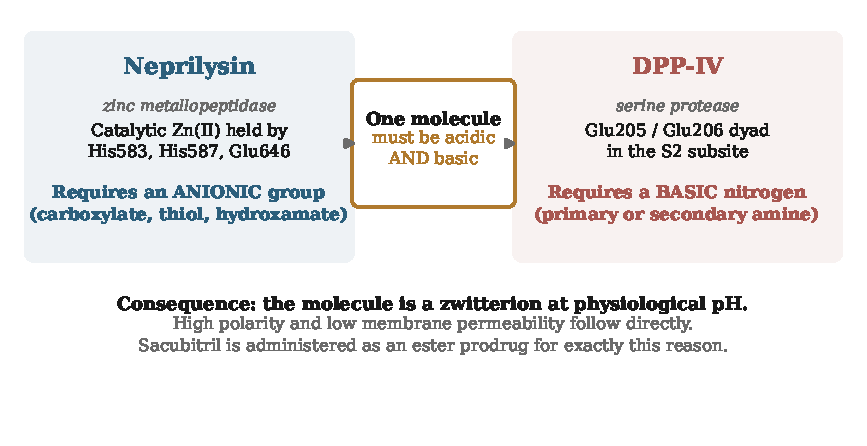
\includegraphics[width=\textwidth]{figs/fig2_pharmacophore.pdf}
\caption{The dual pharmacophore requirement. The two targets demand opposing
ionisable groups. A molecule satisfying both is necessarily zwitterionic, which
carries a direct permeability cost. This is a chemical constraint the pipeline
must work within rather than a problem it can solve.}
\end{figure}

Zwitterions are poorly membrane-permeant. The practical evidence sits in the
clinic already: sacubitril is dosed as an ethyl ester prodrug precisely because
its active carboxylate form does not adequately cross membranes.

This does not make the project impossible. It makes the project honest about
what it is looking for. Three outcomes are plausible.

\begin{enumerate}
\item A zwitterionic molecule with adequate permeability, most likely small and
conformationally constrained, possibly exploiting an intramolecular hydrogen
bond to mask polarity.
\item A prodrug strategy, masking the acid as an ester and relying on
esterase-mediated activation, following the sacubitril precedent.
\item A molecule using a neutral zinc-binding group such as a hydroxamate,
trading some neprilysin potency for improved physical properties.
\end{enumerate}

A screening campaign that does not state this constraint up front will discover
it expensively, several months in, when the surviving compounds all turn out to
be undevelopable.

\section{Hypothesis and objectives}

\begin{keybox}
\textbf{Hypothesis.} Within the space of compounds with reported bioactivity
against either neprilysin or DPP-IV, there exist molecular scaffolds capable of
satisfying the binding requirements of both targets simultaneously. Such
scaffolds can be identified computationally by cross-docking, isolated by
scaffold analysis, and elaborated into a focused set of candidates suitable for
experimental testing.
\end{keybox}

The objectives follow directly:

\begin{enumerate}
\item Establish and validate a docking protocol for each target, with
demonstrated ability to discriminate actives from decoys rather than merely to
reproduce a crystal pose.
\item Assemble curated compound libraries for each target from public
bioactivity data.
\item Identify compounds predicted to bind both targets.
\item Extract the molecular scaffolds common to those compounds.
\item Enumerate analogues under an explicit dual-pharmacophore constraint.
\item Eliminate compounds predicted to engage ACE or DPP-8/9.
\item Deliver a prioritised, selectivity-filtered candidate set.
\end{enumerate}

% ======================================================================
\newpage
\part*{Part II \quad Methodology}
\addcontentsline{toc}{part}{Part II: Methodology}

\section{Pipeline overview}

\begin{figure}[htbp]
\centering
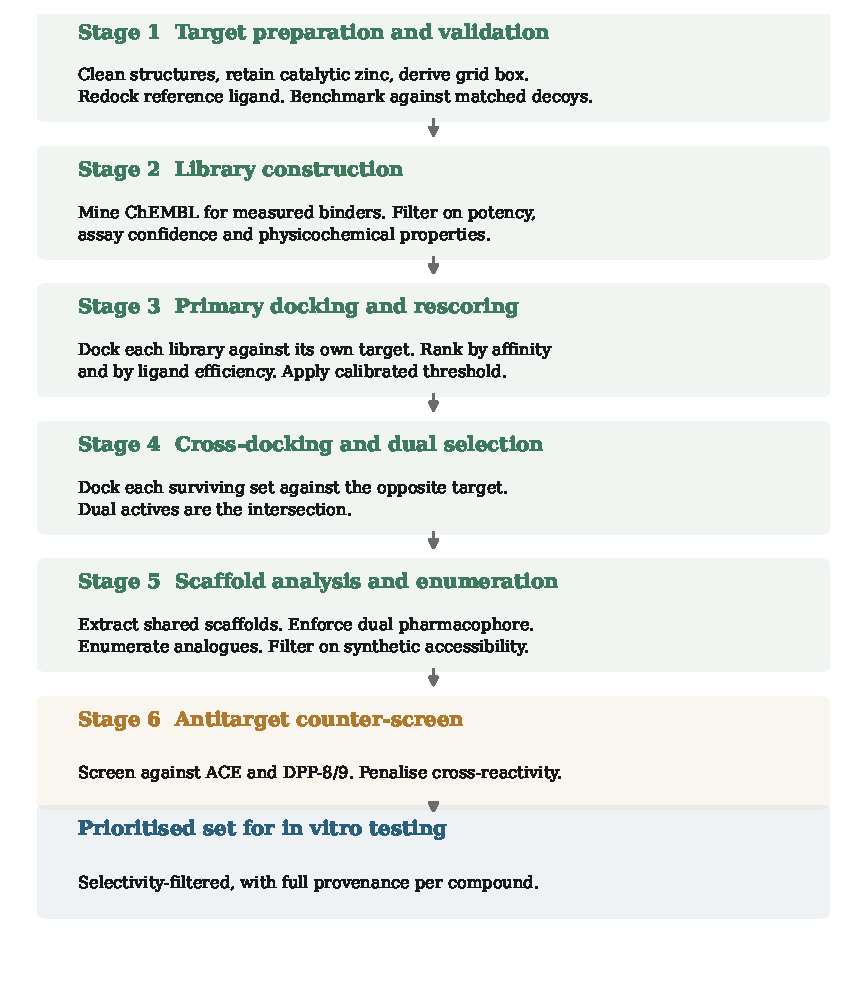
\includegraphics[width=0.93\textwidth]{figs/fig1_pipeline.pdf}
\caption{The complete workflow. Each stage produces a human-readable table and
a provenance record. Stages 1 and 4 act as gates: the pipeline should not
proceed past a failed validation or an empty dual-active set.}
\end{figure}

The design principle throughout is that every stage must produce an inspectable
intermediate and every filter must be justifiable. A virtual screen that cannot
explain why a particular compound survived is not a screen but a lottery with
extra steps.

\section{Stage 1: target preparation}

\subsection{Structure selection}

Suitable structures meet five criteria: human protein; a co-crystallised
inhibitor present (holo rather than apo); resolution 2.5~\ang\ or better; no
missing residues or disordered loops within the binding site; and, for
neprilysin, the catalytic zinc present in the deposited coordinates.

The requirement for a bound ligand is not incidental. The co-crystallised
ligand serves two distinct purposes downstream: it defines the centre of the
docking search box, and it provides the reference pose against which the
protocol is validated. An apo structure provides neither, and its side chains
frequently adopt conformations that no ligand can occupy.

\subsection{Structure preparation}

Preparation removes waters and crystallisation additives, retains one protein
chain, and converts the result to the PDBQT format required by AutoDock.

\begin{warnbox}
\textbf{A failure mode worth naming explicitly.} A routine cleanup step of the
form ``remove all HETATM records'' deletes the catalytic zinc along with the
buffer molecules. Every subsequent calculation then proceeds normally and
produces plausible-looking output that is entirely wrong, because the single
most important feature of the neprilysin binding site is no longer present.

The pipeline maintains a whitelist of functional metal ions, and verifies after
format conversion that the metal survived. A silent failure is converted into a
loud one.
\end{warnbox}

\subsection{Search box definition}

The box centre is the centroid of the co-crystallised ligand. The box
dimensions are taken from configuration, but are enlarged automatically if the
ligand's own bounding box plus 4~\ang\ of padding would exceed them. A box
smaller than the reference ligand cannot reproduce the crystallographic pose,
which would render the validation in Stage 2 meaningless.

\section{Stage 2: protocol validation}

This stage exists to answer a question that is easy to skip and expensive to
skip: does this docking protocol actually work for this target?

\subsection{Redocking}

The co-crystallised ligand is removed, prepared independently, and docked back
into its own site. If the top-ranked pose reproduces the crystallographic pose
to within 2.0~\ang\ root-mean-square deviation, the protocol can at least
reproduce a known answer.

\subsubsection{Symmetry correction in RMSD calculation}

Comparing two poses atom by atom is incorrect whenever the ligand possesses
topological symmetry. The two oxygen atoms of a carboxylate are chemically
indistinguishable; a pose in which they are exchanged is the same pose. A naive
index-based RMSD nevertheless scores such a pose as substantially displaced.

\begin{figure}[htbp]
\centering
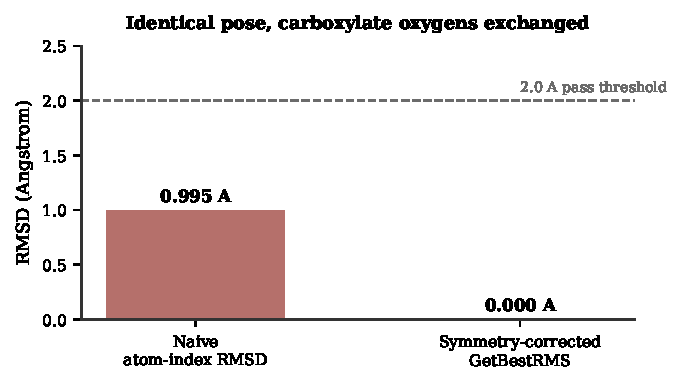
\includegraphics[width=0.62\textwidth]{figs/fig7_rmsd.pdf}
\caption{Measured on a phenylacetic acid in which only the two carboxylate
oxygens are exchanged, leaving the pose chemically identical. Naive atom-index
RMSD reports 0.995~\ang\ of error that does not exist. Symmetry-corrected RMSD
correctly reports zero. For the carboxylate-bearing chemotypes central to
neprilysin inhibition, this difference can determine whether a validation is
reported as a pass or a failure.}
\end{figure}

The pipeline uses a symmetry-corrected RMSD that enumerates substructure
matches and returns the best alignment, and reports the naive value alongside
so that the magnitude of the correction is visible.

\subsection{Enrichment benchmarking}

Redocking demonstrates that a protocol can reproduce a geometry to which it was,
in effect, given the answer. It says nothing about whether the protocol can
rank an active compound above an inactive one, which is the only thing a virtual
screen actually does.

The enrichment benchmark addresses this. Known actives are mixed with decoys,
the mixture is docked, and the extent to which actives rise to the top of the
ranking is measured.

\subsubsection{Why decoys must be property-matched}

If decoys were drawn at random, they would differ from the actives in molecular
weight, charge and lipophilicity. Docking would then separate the two sets on
those trivial grounds, producing excellent apparent enrichment that reflects
nothing about binding. This is the construction principle behind the DUD-E
benchmark set \cite{mysinger2012}.

Each decoy is therefore matched to an active within tolerance on six
properties, while being constrained to remain topologically dissimilar so that
a genuine active cannot enter the decoy set by accident.

\begin{table}[htbp]
\centering
\small
\caption{Decoy matching criteria. The property tolerances remove the trivial
discriminators; the similarity ceiling prevents true actives contaminating the
decoy set.}
\begin{tabular}{lll}
\toprule
\textbf{Criterion} & \textbf{Tolerance} & \textbf{Purpose} \\
\midrule
Molecular weight & $\pm$ 25 Da & remove size as a discriminator \\
Calculated logP & $\pm$ 1.0 & remove lipophilicity as a discriminator \\
H-bond donors & $\pm$ 1 & match polarity profile \\
H-bond acceptors & $\pm$ 2 & match polarity profile \\
Rotatable bonds & $\pm$ 2 & match flexibility \\
Formal charge & exact & charge state strongly affects docking \\
\midrule
Tanimoto similarity & $\leq$ 0.35 & exclude probable true actives \\
\bottomrule
\end{tabular}
\end{table}

\subsubsection{Metrics and their interpretation}

\begin{figure}[htbp]
\centering
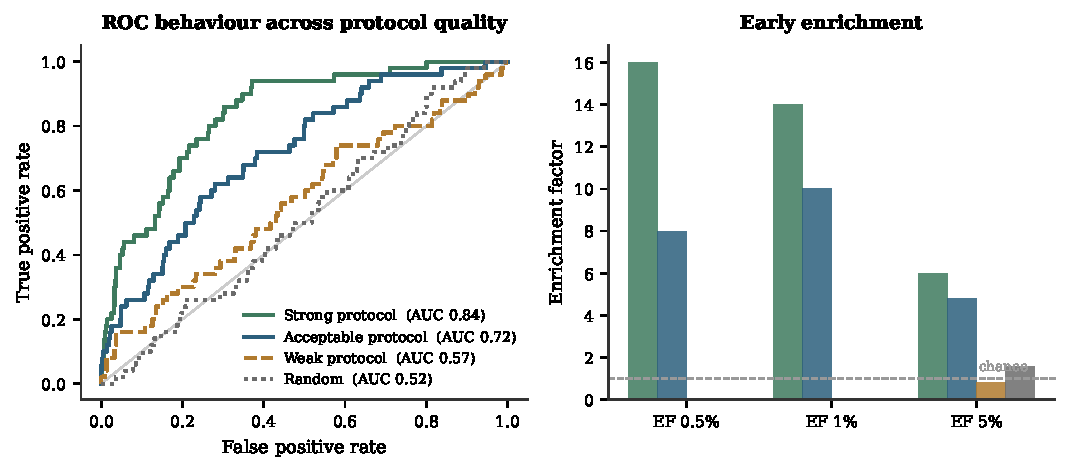
\includegraphics[width=\textwidth]{figs/fig3_roc.pdf}
\caption{Illustrative benchmark behaviour across four protocol qualities,
computed on simulated score distributions with 50 actives among 1000 compounds.
Left: receiver operating characteristic curves. Right: enrichment factors at
three list depths. Note that enrichment factor has a ceiling set by the
total-to-active ratio, here 20. These values demonstrate how the metrics
respond and are not measurements from this project.}
\end{figure}

\begin{table}[htbp]
\centering
\small
\caption{Interpreting the enrichment benchmark.}
\begin{tabular}{p{2.1cm}p{2.5cm}p{9cm}}
\toprule
\textbf{ROC-AUC} & \textbf{Verdict} & \textbf{Action} \\
\midrule
below 0.60 & Unusable & The protocol ranks little better than chance. Screening
with it is an expensive random draw. Revisit preparation, box definition and
metal handling. \\
0.60 to 0.70 & Weak & Usable for coarse triage only. Do not trust the ranking
within the surviving set. \\
0.70 to 0.85 & Acceptable & A normal docking result for a well-behaved target.
Proceed. \\
above 0.85 & Verify first & Unusually strong. Check for a property leak in the
decoy construction before accepting it. \\
\bottomrule
\end{tabular}
\end{table}

Two further points deserve emphasis. First, enrichment factor at 1\% matters
more in practice than ROC-AUC, because compounds are only ever purchased or
synthesised from the top of the ranked list; performance in the tail is
irrelevant. Second, BEDROC with $\alpha = 20$ weights approximately the top 8\%
of the list and is reported for the same reason \cite{truchon2007}.

\subsection{Threshold calibration}

The original project applied a fixed selection threshold of $-9.0$ kcal/mol.
Such a number is typically inherited from a previous publication and carries no
guarantee of appropriateness for a different target or protocol.

This pipeline instead derives the threshold from the benchmark: the score
capturing the desired percentile of the ranked list is computed and written to
the configuration for downstream stages. A cutoff derived from the protocol's
own measured behaviour is defensible in a way that a borrowed constant is not.

\section{Stage 3: library construction}

\subsection{Source and filtering}

Compounds are retrieved from ChEMBL \cite{zdrazil2024}, which aggregates
bioactivity measurements from the primary literature. The aggregation is
valuable and the variation in data quality is considerable, so four filters are
applied at the point of retrieval.

\begin{table}[htbp]
\centering
\small
\caption{Bioactivity filters applied during retrieval. Each discards data
deliberately.}
\begin{tabular}{lll}
\toprule
\textbf{Filter} & \textbf{Setting} & \textbf{Rationale} \\
\midrule
Assay type & Binding (B) & Functional and ADMET readouts measure something else \\
Confidence score & $\geq$ 8 & ChEMBL's own rating of target assignment certainty \\
pChEMBL value & must be present & Guarantees a comparable normalised number \\
Standard relation & equals & Excludes inequalities such as ``greater than 10 uM'' \\
\bottomrule
\end{tabular}
\end{table}

\subsection{Aggregating repeated measurements}

A single compound is frequently measured in several independent studies. These
are collapsed to the median, which resists the single extreme outlier that a
mean would follow.

The range across measurements is retained as a separate field. In testing, a
compound reported at pChEMBL 4.5 in one assay and 9.0 in another was correctly
assigned the median of 6.75 and flagged with a spread of 4.5 log units. A
disagreement of that magnitude means one of the two reports is wrong, and
ChEMBL alone cannot establish which. Such compounds should be treated as
uncertain rather than silently averaged.

\subsection{Chemical standardisation}

The cleaning sequence is fixed and the order is load-bearing:

\begin{center}
parse $\rightarrow$ strip salts $\rightarrow$ standardise $\rightarrow$ reject
PAINS $\rightarrow$ compute properties $\rightarrow$ property filter
$\rightarrow$ deduplicate
\end{center}

\begin{keybox}
\textbf{Why deduplication comes last.} If compounds are deduplicated before
salts are stripped, a hydrochloride salt and its free base are recorded as two
distinct entries and both survive into the library. Stripping first collapses
them to a single compound. This was verified directly: a test set containing
both forms of the same molecule correctly resolved to one entry.
\end{keybox}

\begin{keybox}
\textbf{Why charges are preserved.} Standard cheminformatics practice
neutralises formal charges during standardisation. That practice is wrong for
this project. The dual pharmacophore of Section~\ref{sec:conflict} is
zwitterionic by construction, and neutralising charges would erase precisely the
feature being selected for.
\end{keybox}

PAINS substructures, which produce apparent activity across unrelated assays
through mechanisms unrelated to specific binding, are rejected
\cite{baell2010}.

Physicochemical limits are deliberately looser than the rule of five. A strict
rule-of-five gate would discard the zwitterions this project is looking for.
The filters exclude the clearly undevelopable without prejudging the chemistry.

\subsection{Reporting attrition}

The library builder reports why compounds were rejected, not merely how many
survived. If a large fraction fail on a single property, that property window is
wrong, and the investigator needs to know before committing compute to docking.

\section{Stage 4: primary docking and rescoring}

\subsection{Docking engines}
\label{sec:zincdocking}

AutoDock Vina \cite{trott2010,eberhardt2021} is used for DPP-IV, where it
performs well. It is not used for neprilysin, and the reason is central.

\begin{warnbox}
\textbf{Vina cannot score zinc coordination.} Its scoring function contains no
dedicated term for metal coordination. The catalytic zinc is treated as a
generic atom with van der Waals and electrostatic character, with no
representation of the directional tetrahedral geometry that governs
coordination chemistry.

Since neprilysin inhibition is driven almost entirely by zinc chelation
(Section~2.1), a Vina ranking for this target systematically mis-scores the
single interaction that determines potency.
\end{warnbox}

Neprilysin is therefore docked with AutoDock4 using the AD4Zn force field
\cite{santosmartins2014}, which places four tetrahedrally arranged pseudo-atoms
around the zinc to reproduce its directional coordination preference.

\subsection{Ranking by ligand efficiency}

Raw docking scores scale with molecular size, because a larger molecule makes
more contacts. A ranking by score alone is therefore partly a ranking by
molecular weight, and tends to promote large, lipophilic compounds that are poor
starting points for optimisation.

Ligand efficiency normalises for this:

\begin{equation}
\text{LE} = \frac{-\Delta G_{\text{bind}}}{N_{\text{heavy atoms}}}
\end{equation}

Both rankings are computed and reported. Where they disagree substantially, that
disagreement is itself informative about the composition of the hit set.

\section{Stage 5: cross-docking and dual-activity selection}

Compounds surviving their own target are docked against the opposite target.
Those passing threshold on both constitute the dual-active set.

\subsection{A methodological correction}

The original project bridged the two libraries differently. Each compound in the
neprilysin hit set was compared by two-dimensional Tanimoto similarity against
each compound in the DPP-IV hit set, and only sufficiently similar pairs were
then cross-docked.

This was a reasonable heuristic for saving compute, and it embeds an assumption
that does not hold: that two-dimensional fingerprint similarity implies a shared
binding mode. It does not. Two molecules can be highly similar by fingerprint
and bind entirely differently, or be dissimilar and share a pharmacophore.

Cross-docking the full hit sets in both directions answers the question directly
and removes the assumption. The computational cost is real but modest at the
scale involved, and it is now affordable in a way it was not previously.

\begin{figure}[htbp]
\centering
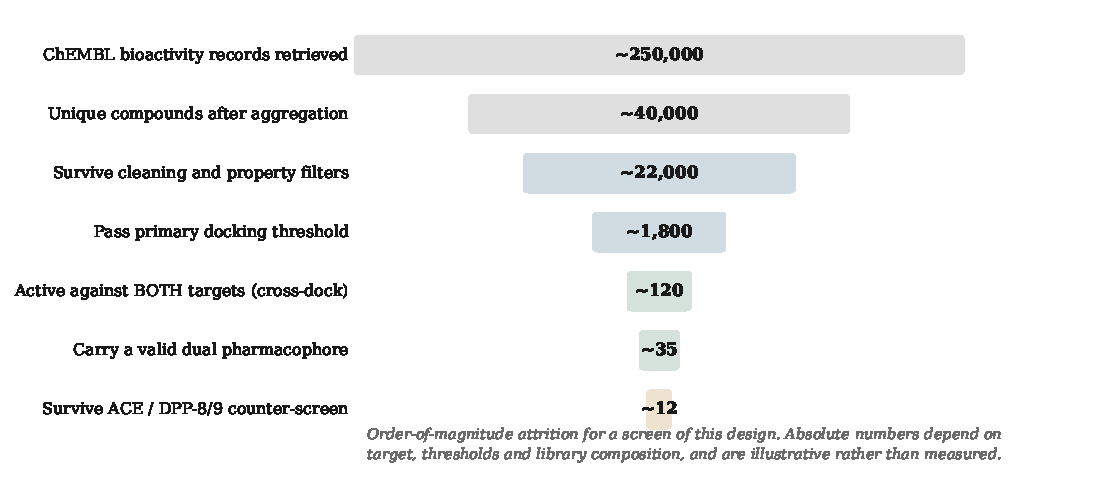
\includegraphics[width=\textwidth]{figs/fig4_funnel.pdf}
\caption{Attrition through the pipeline. The compound count falls by roughly
four orders of magnitude from initial retrieval to the final prioritised set.
The sharpest single drop occurs at the dual-activity intersection, which is the
expected consequence of the pharmacophore conflict described in
Section~\ref{sec:conflict}.}
\end{figure}

\section{Stage 6: scaffold analysis and enumeration}

\subsection{Scaffold extraction}

Molecular scaffolds are extracted using the Bemis and Murcko definition
\cite{bemis1996}: ring systems plus the linkers joining them, with side chains
removed. Scaffolds are ranked by how frequently they recur across the
dual-active set.

In the original project, the scaffolds carried forward were selected manually by
the project supervisor. Expert selection is legitimate, but it is not
reproducible by a third party. This pipeline ranks scaffolds by explicit
criteria, which makes the selection auditable.

\subsection{The dual-pharmacophore constraint}

This is the point at which the analysis of Section~\ref{sec:conflict} becomes an
executable filter rather than a background observation. Scaffolds must carry
both required features, expressed as SMARTS substructure patterns:

\begin{table}[htbp]
\centering
\small
\caption{The dual-pharmacophore constraint, expressed as substructure queries.
A scaffold must match at least one pattern from each group.}
\begin{tabular}{llp{6.6cm}}
\toprule
\textbf{Target} & \textbf{Feature} & \textbf{SMARTS} \\
\midrule
NEP & carboxylate & \texttt{[CX3](=O)[OX1H0-,OX2H1]} \\
NEP & hydroxamate & \texttt{[CX3](=O)[NX3][OX2H1]} \\
NEP & thiol & \texttt{[SX2H]} \\
NEP & phosphinate & \texttt{[PX4](=O)([OX1H0-,OX2H1])} \\
\midrule
DPP-IV & primary amine & \texttt{[NX3;H2;!\$(NC=O)]} \\
DPP-IV & secondary amine & \texttt{[NX3;H1;!\$(NC=O);!\$(N-a)]} \\
\bottomrule
\end{tabular}
\end{table}

Making the requirement explicit converts a hope into a specification. It also
makes subsequent failures interpretable: if no scaffold satisfies both patterns,
that is a meaningful negative result about the accessible chemical space, not an
unexplained empty output.

\subsection{Analogue enumeration}

Selected scaffolds are elaborated into analogue sets. The original project used
DataWarrior for this, which works but introduces a graphical step into an
otherwise scriptable pipeline and therefore breaks end-to-end reproducibility.
Enumeration here is performed programmatically.

Enumerated structures are filtered on synthetic accessibility
\cite{ertl2009}. Unconstrained enumeration generates large numbers of
structures that are formally valid and practically unmakeable, and filtering
them early avoids wasting docking capacity on molecules no chemist could
deliver.

\section{Stage 7: antitarget counter-screening}
\label{sec:counterscreen}

Surviving compounds are docked against the antitargets identified in Section~4.

\begin{table}[htbp]
\centering
\small
\caption{Antitarget panel and the clinical evidence motivating each.}
\begin{tabular}{llp{8.2cm}}
\toprule
\textbf{Antitarget} & \textbf{Relevance} & \textbf{Evidence} \\
\midrule
ACE & NEP-linked & Dual NEP/ACE inhibition by omapatrilat caused angioedema at
2.17\% versus 0.68\% for enalapril in OCTAVE, preventing approval
\cite{kostis2004,packer2002}. \\
\addlinespace
DPP-8 / DPP-9 & DPP-IV-linked & Non-selective inhibition produced alopecia,
thrombocytopenia, reticulocytopenia, splenomegaly, multi-organ pathology and
mortality in rodents, and gastrointestinal toxicity in dogs
\cite{lankas2005}. \\
\bottomrule
\end{tabular}
\end{table}

Compounds scoring well against an antitarget are penalised rather than
discarded outright, since the selectivity margin is itself a property to be
optimised rather than a binary gate.

% ======================================================================
\newpage
\part*{Part III \quad The Machine Learning Component}
\addcontentsline{toc}{part}{Part III: The Machine Learning Component}

\section{Machine learning in this pipeline}
\label{sec:ml}

\begin{keybox}
\textbf{Attribution.} In the original project, this component was implemented by
a doctoral colleague rather than by the present author. It is described here in
full so that the pipeline can be reproduced end to end, and because the
methodological issues it raises are instructive and widely shared.
\end{keybox}

\subsection{What problem the model is solving}

By the end of Stage 6, enumeration has produced tens of thousands of candidate
structures. Docking all of them is feasible but slow, and docking is itself only
an approximation. The purpose of the model is triage: to learn the relationship
between molecular structure and predicted activity from the compounds already
scored, and then to prioritise the remainder without docking each one.

This is a supervised regression problem. The input is a molecule. The output is
a number representing predicted activity. The model learns the mapping from
examples.

\subsection{Representing a molecule as numbers}

A machine learning model cannot read a chemical structure directly. The molecule
must be converted into a fixed-length numeric vector, a process called
featurisation. Three approaches are common.

\subsubsection{Molecular descriptors}

The simplest option. Compute a set of interpretable numbers for each molecule:
molecular weight, calculated logP, topological polar surface area, counts of
hydrogen bond donors and acceptors, rotatable bonds, ring counts, and so on. A
few hundred such descriptors are readily available.

Strengths: interpretable, cheap, robust with small datasets. Weakness: two
molecules with very different structures can share almost identical descriptor
profiles, so the representation discards structural information the model may
need.

\subsubsection{Fingerprints}

The standard approach in this domain. An extended-connectivity fingerprint
(ECFP) examines the local environment of every atom out to a fixed bond radius,
hashes each environment into an integer, and sets the corresponding bit in a
fixed-length vector \cite{rogers2010}. ECFP4, meaning radius 2, in 2048 bits is
the usual default.

The result is a binary vector in which each position indicates the presence or
absence of a particular substructural motif. Similar molecules share many bits.
This representation is cheap, deterministic, and empirically hard to beat on
datasets of the size typically available in a project like this one.

\subsubsection{Learned representations}

Graph neural networks treat the molecule as a graph of atoms and bonds and learn
the featurisation jointly with the prediction task. This is the modern approach
and can outperform fingerprints, but it requires substantially more data to
train well. On a few thousand compounds it typically does not beat a
well-tuned gradient boosting model on ECFP4.

\begin{keybox}
\textbf{Practical recommendation.} Start with ECFP4 concatenated with a
handful of physicochemical descriptors. It is a strong baseline that is
difficult to beat on datasets below roughly ten thousand compounds, and it
establishes whether a more complex model is earning its complexity.
\end{keybox}

\subsection{The label problem}

This is the most important section in Part III, and the point on which the
original project can be most usefully criticised.

A supervised model learns to predict whatever it is trained on. The choice of
label therefore determines what the model actually learns, and no amount of
architectural sophistication can compensate for the wrong choice.

The original model was trained on docking scores. The reasoning was practical:
docking scores were available for every enumerated compound, and experimental
data was not available for most of them.

\begin{warnbox}
\textbf{The consequence.} A model trained on docking scores learns to
approximate the scoring function, not the biology. Its accuracy ceiling is the
accuracy of the docking programme it was trained against. A model that
reproduced Vina perfectly would inherit every one of Vina's errors, including
the systematic mis-scoring of zinc coordination described in
Section~\ref{sec:zincdocking}.
\end{warnbox}

\begin{figure}[htbp]
\centering
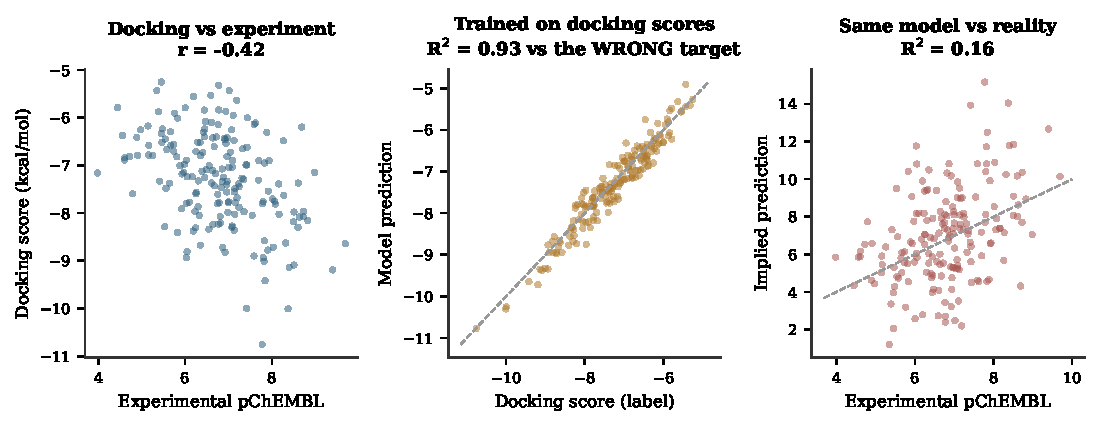
\includegraphics[width=\textwidth]{figs/fig5_ml.pdf}
\caption{Why the label choice dominates. Left: docking scores correlate only
weakly with experimental potency, which is a well-documented property of
docking rather than a defect of any particular implementation. Centre: a model
trained on docking scores can reproduce them with high fidelity. Right: that
same model, evaluated against experimental potency, performs poorly. The model
is excellent at the task it was given and the task was the wrong one.
Simulated data illustrating the structure of the problem.}
\end{figure}

\subsubsection{The data that was already available}

The better approach required no additional experiments and no additional
compute. Stage 3 of this pipeline mines ChEMBL for compounds \emph{filtered by
their measured IC50 values}. Those experimental potency labels were downloaded
in order to apply the filter, and were then discarded in favour of computed
scores.

A model trained on experimental pChEMBL values for both targets would have used
data that was already in hand. The docking scores could still contribute, as an
auxiliary prediction task or as a pre-training signal, without being treated as
ground truth.

\subsection{Multi-task architecture}

Because the project needs predictions for two targets, the natural design shares
most of the model between them.

\begin{figure}[htbp]
\centering
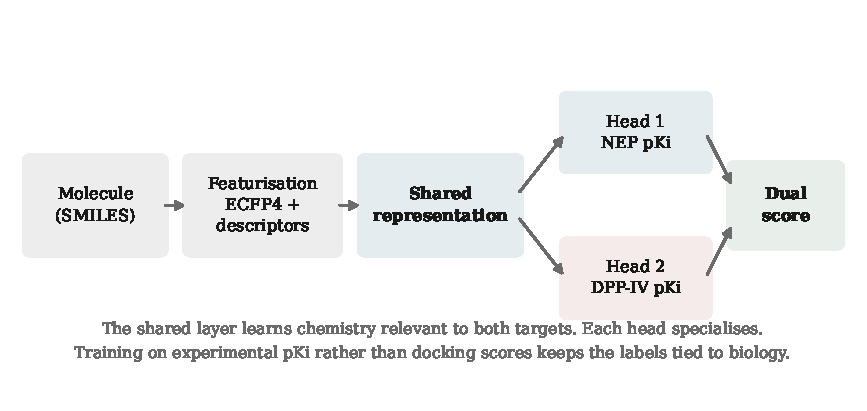
\includegraphics[width=\textwidth]{figs/fig6_multitask.pdf}
\caption{Multi-task architecture. A shared representation learns chemistry
relevant to both targets, while separate output heads specialise. Training on
experimental potency keeps the labels tied to biology rather than to a scoring
function.}
\end{figure}

The reasoning is that binding to either target depends on overlapping chemical
properties: shape, lipophilicity, hydrogen bonding capacity, charge
distribution. A shared layer can learn these once from the combined data of both
targets, which is particularly valuable when one target has substantially fewer
measurements than the other.

\subsection{Choosing a model}

\begin{table}[htbp]
\centering
\small
\caption{Model selection for datasets of the size typical in this setting.}
\begin{tabular}{lp{4.4cm}p{5.6cm}}
\toprule
\textbf{Model} & \textbf{When to use} & \textbf{Notes} \\
\midrule
Random Forest & First baseline & Almost impossible to configure badly. If a more
complex model cannot beat it, the complexity is not earning its place. \\
\addlinespace
Gradient boosting (XGBoost, LightGBM) & Default choice & Usually the best
performer on fingerprint input at this scale \cite{chen2016}. Handles sparse
binary features well. \\
\addlinespace
Neural network (MLP) & Multi-task settings & The natural choice when a shared
representation with multiple heads is wanted. \\
\addlinespace
Graph neural network & Large datasets & Requires more data than this kind of
project usually has. Worth revisiting above roughly ten thousand measured
compounds. \\
\bottomrule
\end{tabular}
\end{table}

\subsection{Validation: the part that is most often done wrong}

A model that performs well on data resembling its training set may perform very
poorly on genuinely novel chemistry. Since the purpose here is to prioritise
\emph{new} compounds, the evaluation must reflect that.

\subsubsection{Why random splitting overestimates performance}

Chemical datasets contain congeneric series: groups of closely related analogues
from the same medicinal chemistry programme. A random train/test split places
some members of a series in training and others in test. The model then
predicts a compound nearly identical to one it has already seen, and appears
highly accurate.

\subsubsection{Scaffold splitting}

The correct approach for this application is to split by scaffold, so that all
compounds sharing a Bemis-Murcko scaffold fall on the same side of the split.
The test set then contains chemotypes the model has genuinely not encountered,
which is the situation it will face in deployment.

\begin{keybox}
\textbf{Expect the number to fall.} A model scoring $R^2 = 0.85$ under random
splitting may score $0.45$ under scaffold splitting. The second number is the
honest one. Report it. A reviewer who sees only the optimistic figure and later
discovers the splitting strategy will discount everything else in the work.
\end{keybox}

\subsubsection{Applicability domain}

A model asked to predict a molecule unlike anything in its training set will
still return a number, and that number will be unreliable. Quantifying the
distance from each prediction to the training distribution, for example through
maximum Tanimoto similarity to any training compound, allows low-confidence
predictions to be flagged rather than silently trusted.

\subsection{A recommended implementation sequence}

\begin{enumerate}
\item Assemble experimental pChEMBL values for both targets from Stage 3 output.
\item Featurise with ECFP4 (2048 bits) plus a small descriptor set.
\item Split by Bemis-Murcko scaffold, approximately 80/20.
\item Train a Random Forest as a baseline and record its scaffold-split
performance.
\item Train a multi-task gradient boosting or neural model with one head per
target.
\item Compare honestly. If the complex model does not beat the baseline, use the
baseline.
\item Compute applicability domain distances for every prediction.
\item Apply the model to enumerated compounds, and dock only the top-ranked
fraction.
\item Report both split strategies, making clear which is which.
\end{enumerate}

% ======================================================================
\newpage
\part*{Part IV \quad Appraisal and Reproduction}
\addcontentsline{toc}{part}{Part IV: Appraisal and Reproduction}

\section{Divergences from the original implementation}

This report describes an improved pipeline. The table below records every point
at which it departs from what was originally done, so that the two are never
confused.

\begin{longtable}{p{2.5cm}p{4.3cm}p{7.6cm}}
\caption{Changes relative to the original undergraduate implementation.}\\
\toprule
\textbf{Stage} & \textbf{Originally} & \textbf{Now, and why} \\
\midrule
\endfirsthead
\toprule
\textbf{Stage} & \textbf{Originally} & \textbf{Now, and why} \\
\midrule
\endhead
Validation & Redocking with visual pose inspection & Redocking retained, plus
enrichment benchmarking against property-matched decoys. Geometric
reproduction does not demonstrate the ability to discriminate actives from
inactives. \\
\addlinespace
NEP docking & AutoDock Vina & AutoDock4 with AD4Zn. Vina has no metal
coordination term, and neprilysin inhibition is driven by zinc chelation. \\
\addlinespace
File preparation & AutoDockTools / MGLTools (Python 2) & Maintained Python 3
equivalents. Output is comparable; the legacy toolchain is effectively
unsupported. \\
\addlinespace
Threshold & Fixed at $-9.0$ kcal/mol & Calibrated from the enrichment
benchmark, with a parallel ligand efficiency ranking to remove the size bias. \\
\addlinespace
Library bridge & 2D Tanimoto similarity, then cross-docking of similar pairs &
Direct cross-docking of both full hit sets. Fingerprint similarity does not
imply a shared binding mode. \\
\addlinespace
Scaffold choice & Manual selection by the supervisor & Frequency-ranked
extraction with an explicit dual-pharmacophore SMARTS filter. Reproducible by a
third party. \\
\addlinespace
Enumeration & DataWarrior (graphical) & Programmatic enumeration with synthetic
accessibility filtering. Keeps the pipeline scriptable end to end. \\
\addlinespace
Antitargets & Not screened & ACE and DPP-8/9 counter-screens added. Given the
omapatrilat precedent these are not optional. \\
\addlinespace
ML labels & Docking scores & Experimental pChEMBL values recommended, with
docking as an auxiliary signal. See Section~\ref{sec:ml}. \\
\bottomrule
\end{longtable}

\section{Limitations}

Stated plainly, because a virtual screen that does not state its limitations
should not be trusted.

\begin{enumerate}
\item \textbf{No experimental validation.} No compound described here has been
synthesised or assayed. Everything is prediction.

\item \textbf{Docking scores are weak predictors of affinity.} The correlation
between docking score and measured binding is modest. Scores are used here for
triage and ranking, not as quantitative predictions.

\item \textbf{Receptor flexibility is not modelled.} Docking treats the protein
as rigid. Both targets are known to undergo induced-fit rearrangement on ligand
binding, including a concerted conformational change at Trp693 and Phe106 in
neprilysin when a bulky group occupies the S1' subsite \cite{schiering2016}.

\item \textbf{The zwitterion problem is surfaced, not solved.} The pipeline
identifies molecules satisfying both pharmacophores. It does not make them
permeable.

\item \textbf{Structure-based screening finds what resembles what is known.}
Libraries are built from compounds with reported activity, which biases the
search toward established chemotypes.

\item \textbf{Absolute numbers in this report are illustrative.} Figures
demonstrating metric behaviour use simulated data, and this is stated in every
relevant caption.
\end{enumerate}

\section{Reproducing this work}

\subsection{Prerequisites}

\begin{table}[htbp]
\centering
\small
\caption{Software requirements.}
\begin{tabular}{lll}
\toprule
\textbf{Component} & \textbf{Purpose} & \textbf{Availability} \\
\midrule
RDKit & Cheminformatics throughout & conda-forge, open source \\
AutoDock Vina 1.2 & Docking (DPP-IV) & conda-forge, open source \\
AutoDock4 + AD4Zn & Docking (NEP, zinc-aware) & Scripps, free \\
Open Babel & Format conversion & conda-forge, open source \\
ADFR Suite & Receptor preparation & Scripps, free \\
scikit-learn & Metrics and baseline models & conda-forge, open source \\
ChEMBL & Bioactivity source & Public REST API \\
\bottomrule
\end{tabular}
\end{table}

\subsection{Procedure}

\begin{enumerate}
\item Select and verify target structures against the criteria in Section~8.1.
Record the accession codes, chains and ligand codes chosen, and the reasons.

\item Prepare the receptors, retaining the catalytic zinc. Confirm it survived
format conversion.

\item Validate. Redock the reference ligands, using symmetry-corrected RMSD.
Then build a property-matched decoy set and measure ROC-AUC and enrichment. Do
not proceed past a failing validation.

\item Build the libraries from ChEMBL with the filters in Section~10, and
inspect the attrition report before continuing.

\item Dock each library against its own target. Rank by affinity and by ligand
efficiency.

\item Cross-dock in both directions. Take the intersection as the dual-active
set.

\item Extract scaffolds, apply the dual-pharmacophore SMARTS filter, enumerate
analogues, and filter on synthetic accessibility.

\item Counter-screen against ACE and DPP-8/9.

\item If applying machine learning, follow Section~\ref{sec:ml}, and use
experimental labels with scaffold-based splitting.
\end{enumerate}

\subsection{Compute}

A full-scale campaign of the order of $10^5$ compounds per target requires
several thousand CPU-hours and is intended for cluster execution. Every stage
accepts a limit argument that truncates the working set, allowing the complete
workflow to be exercised on a laptop before committing to a full run. Running
the reduced version first is strongly advised; errors in grid definition or
receptor preparation are considerably cheaper to discover at that scale.

\section{Concluding remarks}

The scientific contribution of this work is a reproducible protocol rather than
a compound. Its more useful lesson is methodological.

Two of the defects identified here, the absence of enrichment benchmarking and
the use of docking scores as machine learning labels, are not unusual. They
appear regularly in published virtual screening studies. Both produce work that
looks entirely normal and is substantially less informative than it appears,
which is precisely what makes them worth naming.

The pharmacophore conflict at the centre of this project is genuine and
unresolved. A molecule that inhibits both neprilysin and DPP-IV must carry
opposing ionisable groups, and will pay for that in permeability. The pipeline
described here is capable of finding such molecules. Whether any of them can be
developed into a drug is a question that computation is not equipped to answer,
and that only synthesis and assay can settle.

% ======================================================================
\newpage
\begin{thebibliography}{99}
\small

\bibitem{packer2002}
Packer M, Califf RM, Konstam MA, et al.
Comparison of omapatrilat and enalapril in patients with chronic heart failure:
the Omapatrilat Versus Enalapril Randomized Trial of Utility in Reducing Events
(OVERTURE). \textit{Circulation} 2002;106:920--926.

\bibitem{kostis2004}
Kostis JB, Packer M, Black HR, et al.
Omapatrilat and enalapril in patients with hypertension: the Omapatrilat
Cardiovascular Treatment vs. Enalapril (OCTAVE) trial.
\textit{American Journal of Hypertension} 2004;17:103--111.

\bibitem{lankas2005}
Lankas GR, Leiting B, Sinha Roy R, et al.
Dipeptidyl peptidase IV inhibition for the treatment of type 2 diabetes:
potential importance of selectivity over dipeptidyl peptidases 8 and 9.
\textit{Diabetes} 2005;54:2988--2994.

\bibitem{schiering2016}
Schiering N, D'Arcy A, Villard F, et al.
Structure of neprilysin in complex with the active metabolite of sacubitril.
\textit{Scientific Reports} 2016;6:27909.

\bibitem{kim2005}
Kim D, Wang L, Beconi M, et al.
(2R)-4-oxo-4-[3-(trifluoromethyl)-5,6-dihydro[1,2,4]triazolo[4,3-a]pyrazin-7(8H)-yl]-1-(2,4,5-trifluorophenyl)butan-2-amine:
a potent, orally active dipeptidyl peptidase IV inhibitor for the treatment of
type 2 diabetes. \textit{Journal of Medicinal Chemistry} 2005;48:141--151.
(PDB entry 1X70.)

\bibitem{trott2010}
Trott O, Olson AJ.
AutoDock Vina: improving the speed and accuracy of docking with a new scoring
function, efficient optimization, and multithreading.
\textit{Journal of Computational Chemistry} 2010;31:455--461.

\bibitem{eberhardt2021}
Eberhardt J, Santos-Martins D, Tillack AF, Forli S.
AutoDock Vina 1.2.0: new docking methods, expanded force field, and Python
bindings. \textit{Journal of Chemical Information and Modeling}
2021;61:3891--3898.

\bibitem{santosmartins2014}
Santos-Martins D, Forli S, Ramos MJ, Olson AJ.
AutoDock4$_{\text{Zn}}$: an improved AutoDock force field for small-molecule
docking to zinc metalloproteins.
\textit{Journal of Chemical Information and Modeling} 2014;54:2371--2379.

\bibitem{mysinger2012}
Mysinger MM, Carchia M, Irwin JJ, Shoichet BK.
Directory of Useful Decoys, Enhanced (DUD-E): better ligands and decoys for
better benchmarking.
\textit{Journal of Medicinal Chemistry} 2012;55:6582--6594.

\bibitem{truchon2007}
Truchon JF, Bayly CI.
Evaluating virtual screening methods: good and bad metrics for the ``early
recognition'' problem.
\textit{Journal of Chemical Information and Modeling} 2007;47:488--508.

\bibitem{zdrazil2024}
Zdrazil B, Felix E, Hunter F, et al.
The ChEMBL Database in 2023: a drug discovery platform spanning multiple
bioactivity data types and time periods.
\textit{Nucleic Acids Research} 2024;52:D1180--D1192.

\bibitem{rogers2010}
Rogers D, Hahn M.
Extended-connectivity fingerprints.
\textit{Journal of Chemical Information and Modeling} 2010;50:742--754.

\bibitem{bemis1996}
Bemis GW, Murcko MA.
The properties of known drugs. 1. Molecular frameworks.
\textit{Journal of Medicinal Chemistry} 1996;39:2887--2893.

\bibitem{baell2010}
Baell JB, Holloway GA.
New substructure filters for removal of pan assay interference compounds
(PAINS) from screening libraries and for their exclusion in bioassays.
\textit{Journal of Medicinal Chemistry} 2010;53:2719--2740.

\bibitem{ertl2009}
Ertl P, Schuffenhauer A.
Estimation of synthetic accessibility score of drug-like molecules based on
molecular complexity and fragment contributions.
\textit{Journal of Cheminformatics} 2009;1:8.

\bibitem{chen2016}
Chen T, Guestrin C.
XGBoost: a scalable tree boosting system.
\textit{Proceedings of the 22nd ACM SIGKDD International Conference on Knowledge
Discovery and Data Mining} 2016:785--794.

\end{thebibliography}

\vspace{0.6cm}
\noindent{\footnotesize\color{soft}
Bibliographic details should be verified against the primary sources before
formal citation. Software tools invoked by the pipeline carry their own
licensing and citation requirements, listed in the accompanying repository.}

\end{document}
